\subsection{Figures and Tables}

\begin{figure}[H]
  \label{compute-times}
  \caption{Compute times for various approximation configurations.}
  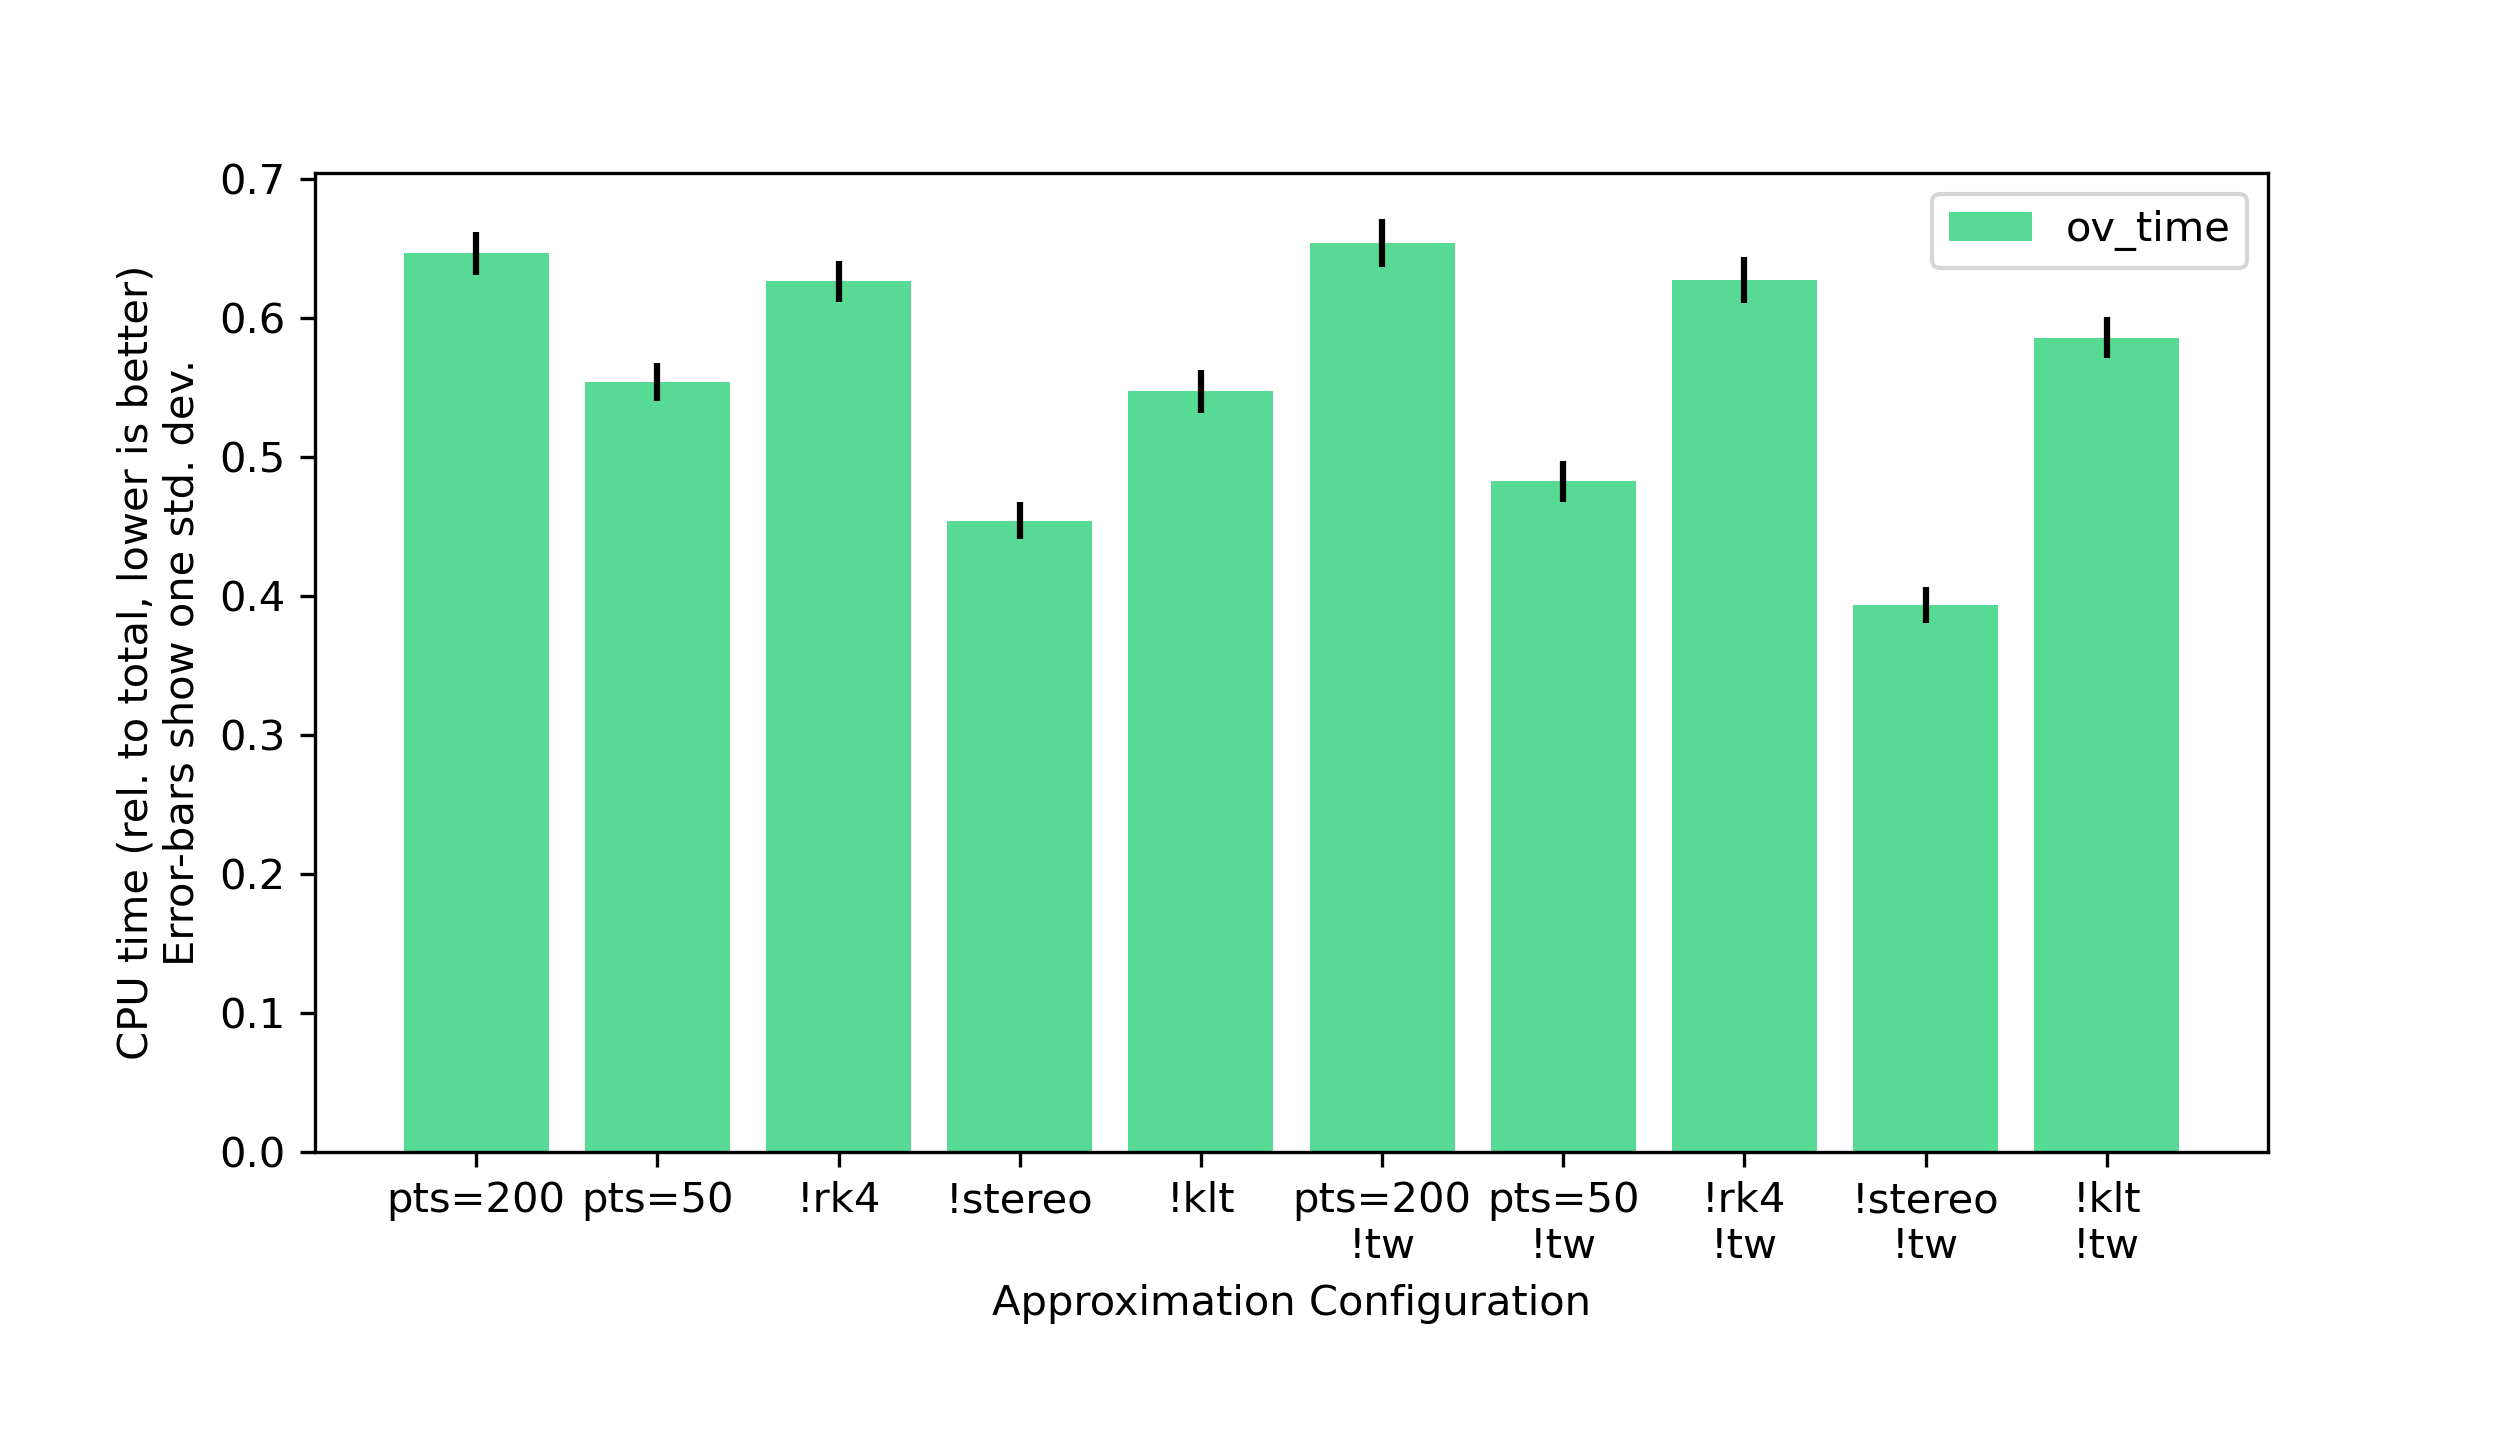
\includegraphics[width=\columnwidth]{times.png}
\end{figure}

\begin{table*}
  \centering
  {
    \caption{OpenVINS approximation knobs. See OpenVINS documentation for more details\cite{Geneva2020ICRA}.}
    \begin{tabularx}{\linewidth}{r||l|X}
      \textbf{Knob} & \textbf{Range} & \textbf{Meaning} \\
      & {(approx. first)} & \\
      \hline\hline
      \verb+num_pts+ & 50--300 & The number of points extracted and tracked in each image frame \\
      \verb+use_rk4_integration+ & [false, true] & If Rk4 imu integration is used\\
      \verb+use_stereo+ & [false, true] & Whether cameras are stereo or binocular. If binocular, it does monocular feature tracking on each image \\
      \verb+use_klt+ & [false, true] & Uses KLT tracking or descriptor matcher \\
      \verb+downsample_camera+ & [true, false] & Halves the resolution all tracking image \\
      \verb+enable_async_reproject+ & [false, true] & (outside of OpenVINS, elsewhere in ILLIXR) queries a current pose and reprojects the frame just before display, making up for some latency in SLAM \\
    \end{tabularx}
  }
\end{table*}

\begin{figure}[H]
  \label{system-level-errors}
  \caption{System-level error for various approximation configurations.}
  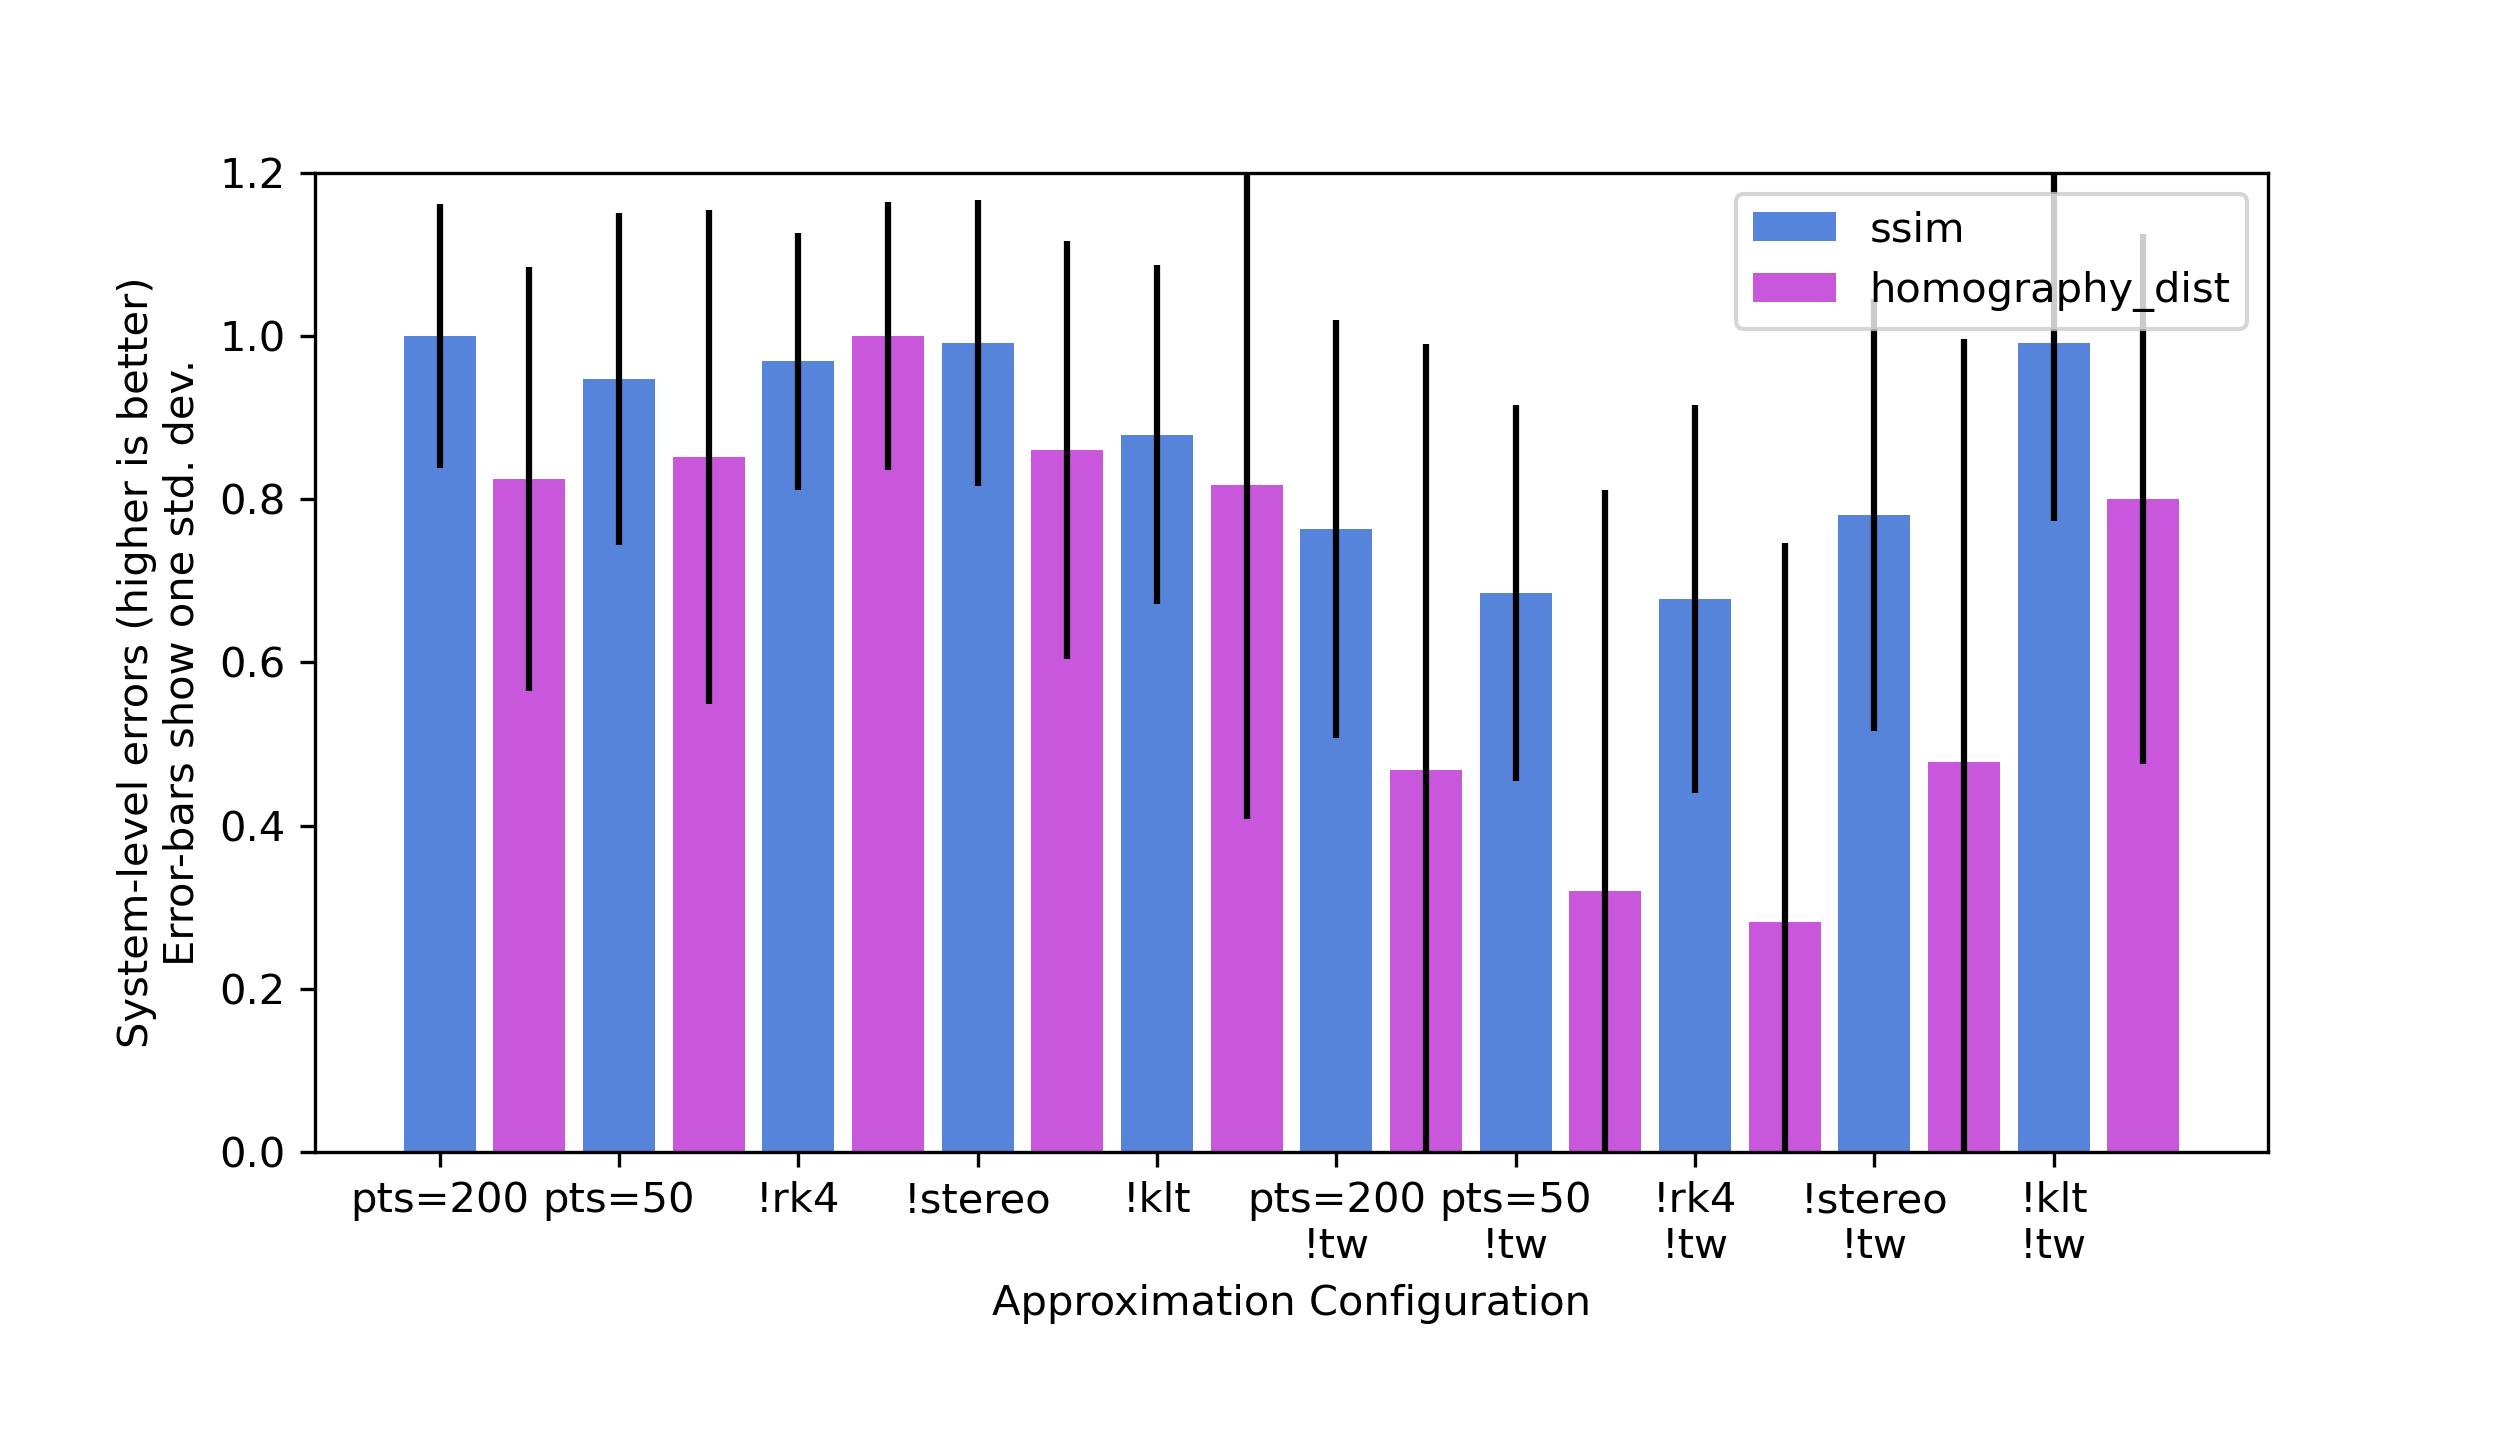
\includegraphics[width=\columnwidth]{system_errors.png}
\end{figure}

\begin{figure}[H]
\caption{AR/VR DAG, showing how SLAM flows to the output over multiple paths.}
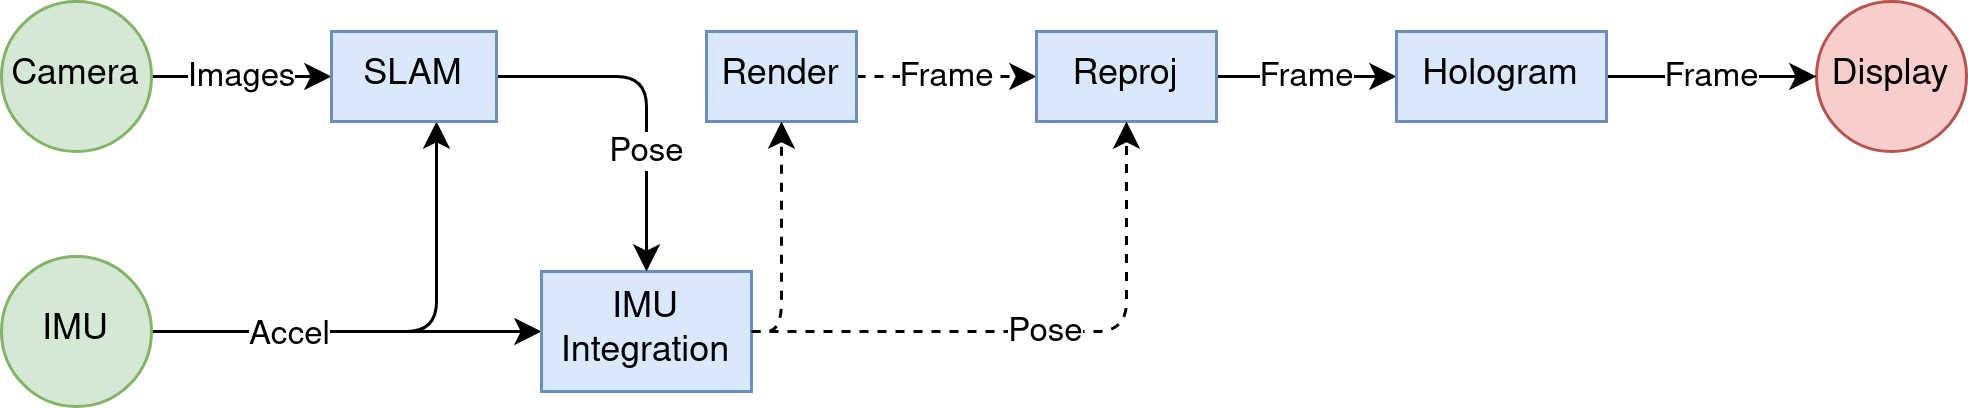
\includegraphics[width=\columnwidth]{dag.png}
\label{dag}
\end{figure}

\begin{figure}[H]
  \label{SLAM-level-errors}
  \caption{SLAM-level error for various approximation configurations.}
  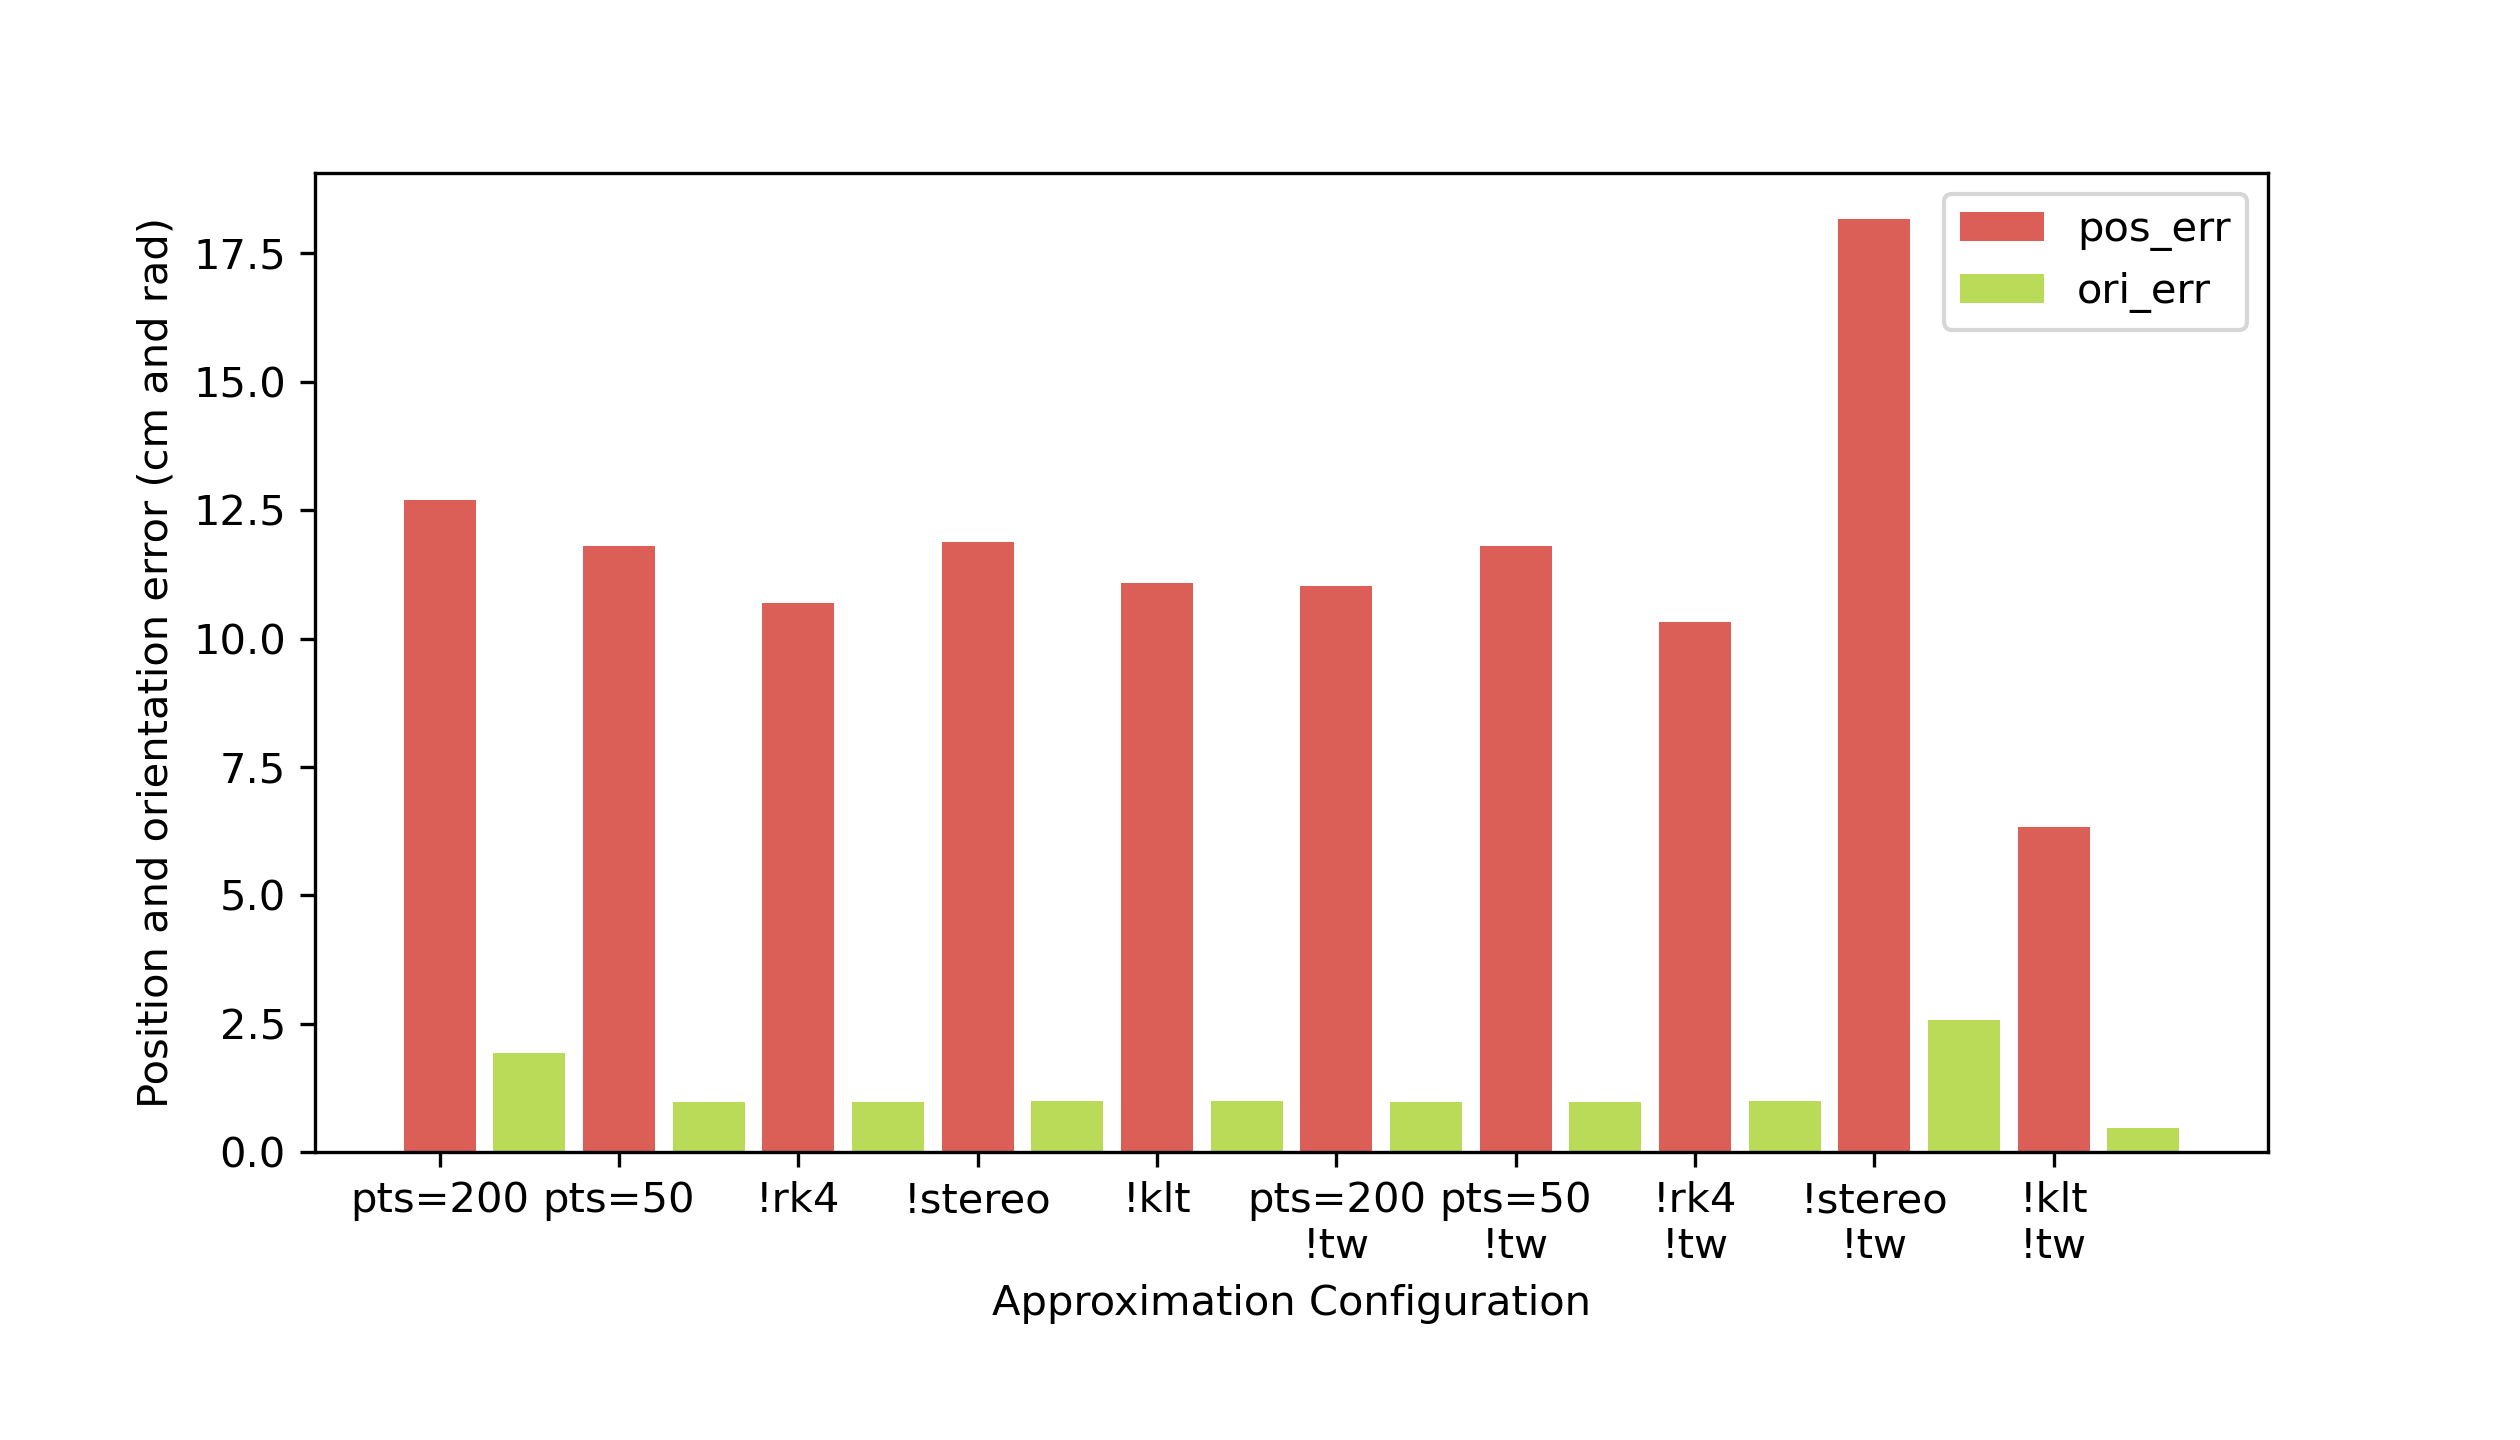
\includegraphics[width=\columnwidth]{slam_errors.png}
\end{figure}

\begin{figure}[H]
  \label{transformation}
  \caption{Unaligned and aligned poses, with dotted arrows showing the transformation}
  \footnote{It only appears that the transformation `distorts' space because the transformation rotates `out of the plane'. This is a 2d projection of a 3d trajectory, so there is a part of the trajectory you can't see.}
  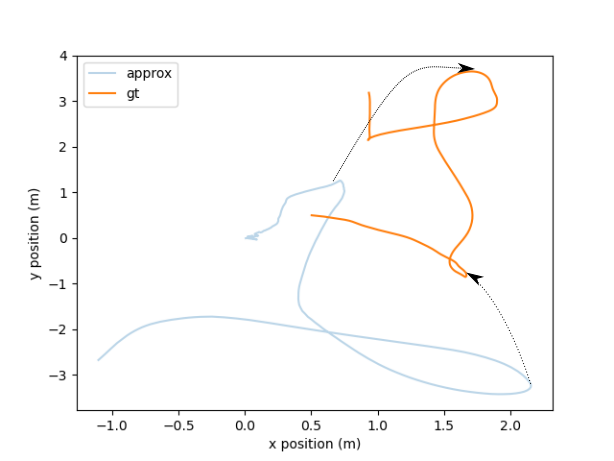
\includegraphics[width=\columnwidth]{unaligned.png}
  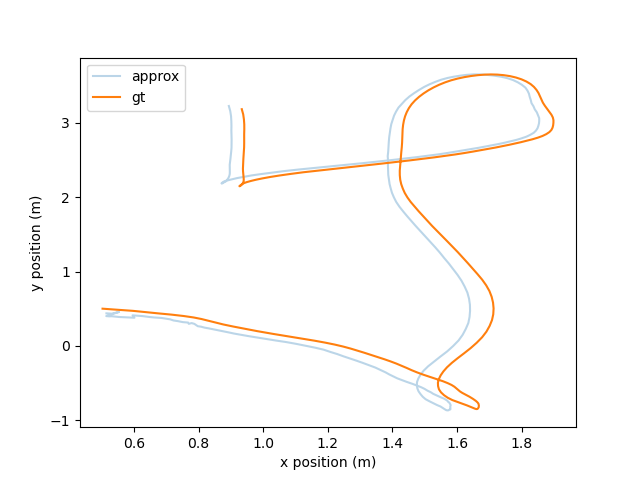
\includegraphics[width=\columnwidth]{aligned.png}
\end{figure}
